\subsubsection{Raman Spectroscopy with Graphene}

\begin{figure}[!h]
  \centering
  \begin{subfigure}{0.45\textwidth}
    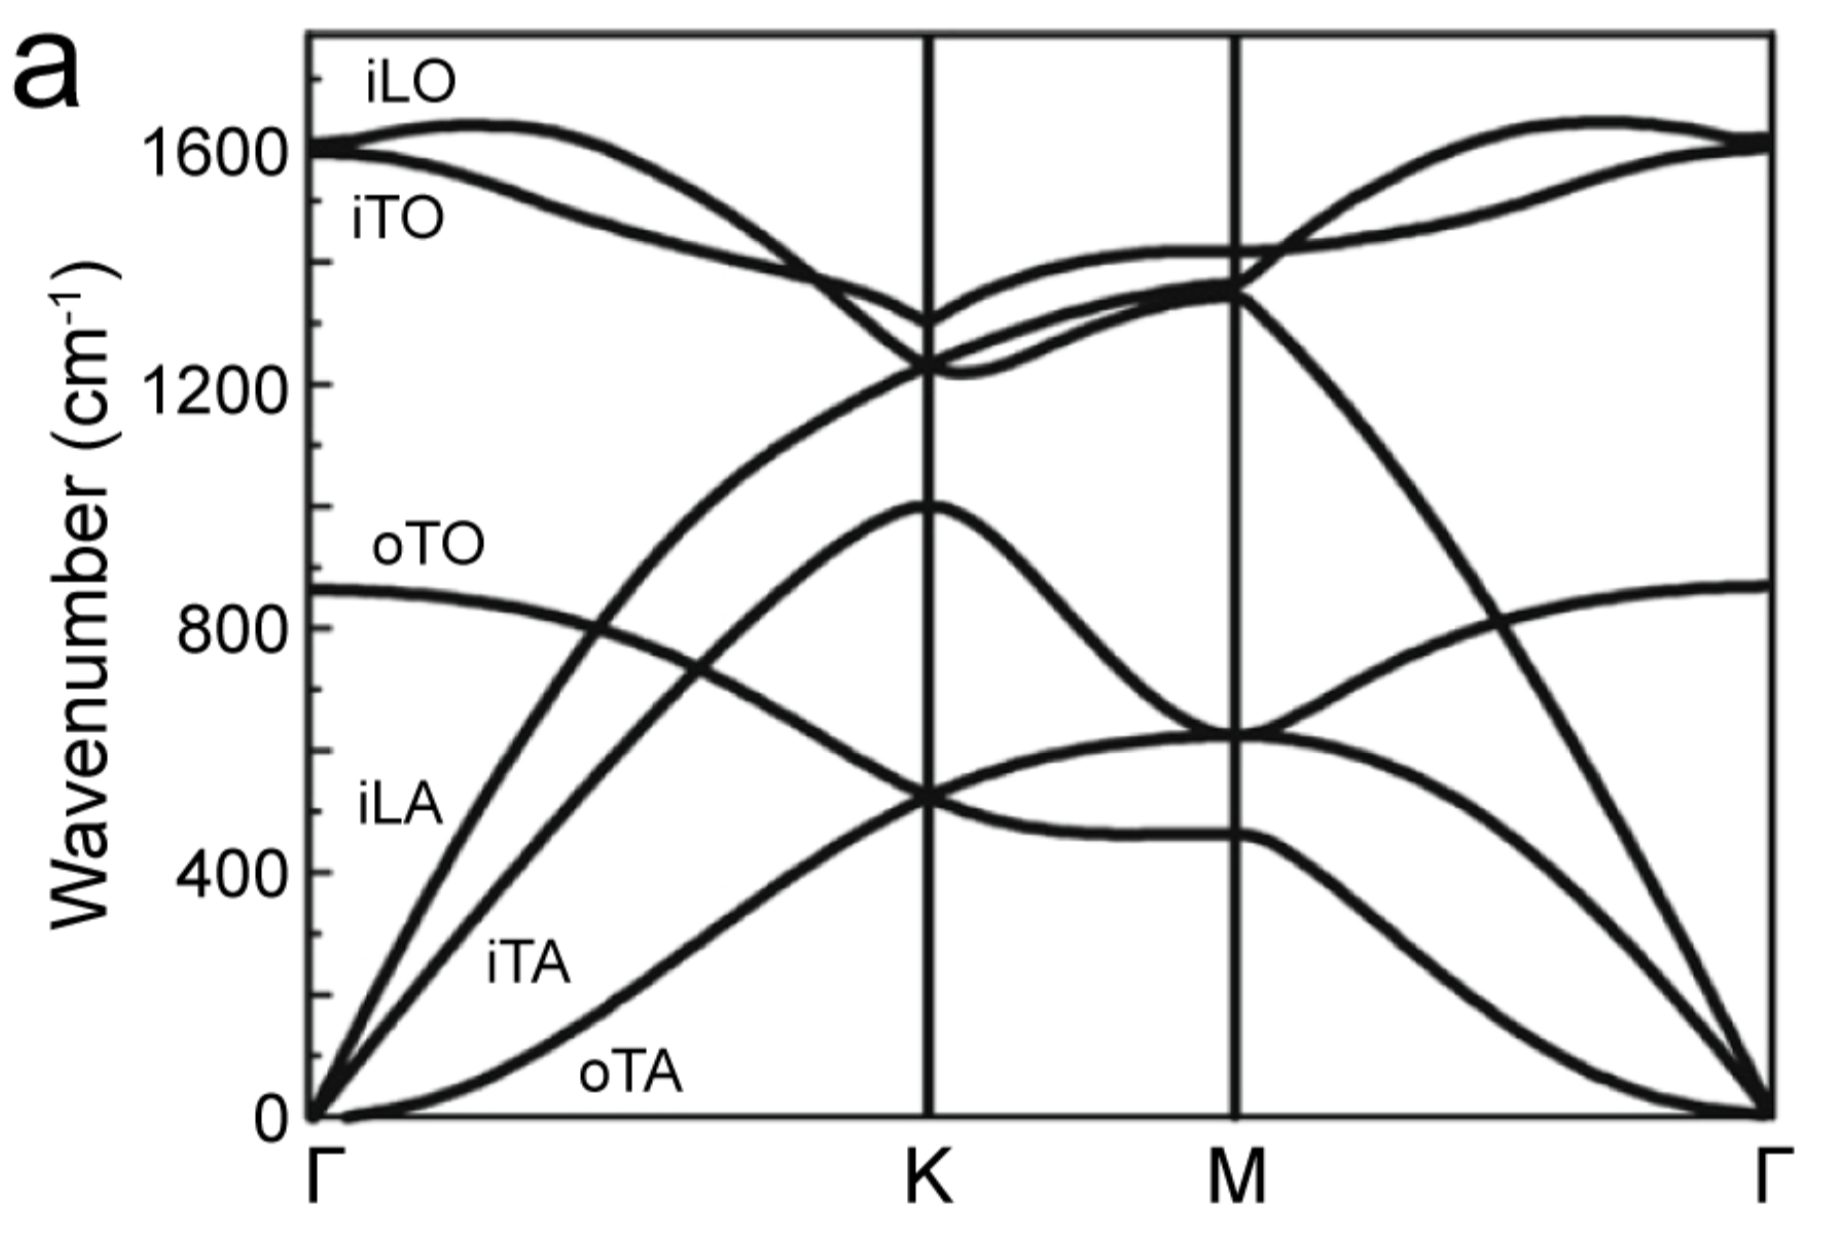
\includegraphics[width=\textwidth]{./images/phonon-modes.png}
  \end{subfigure}
  ~
  \begin{subfigure}{0.45\textwidth}
    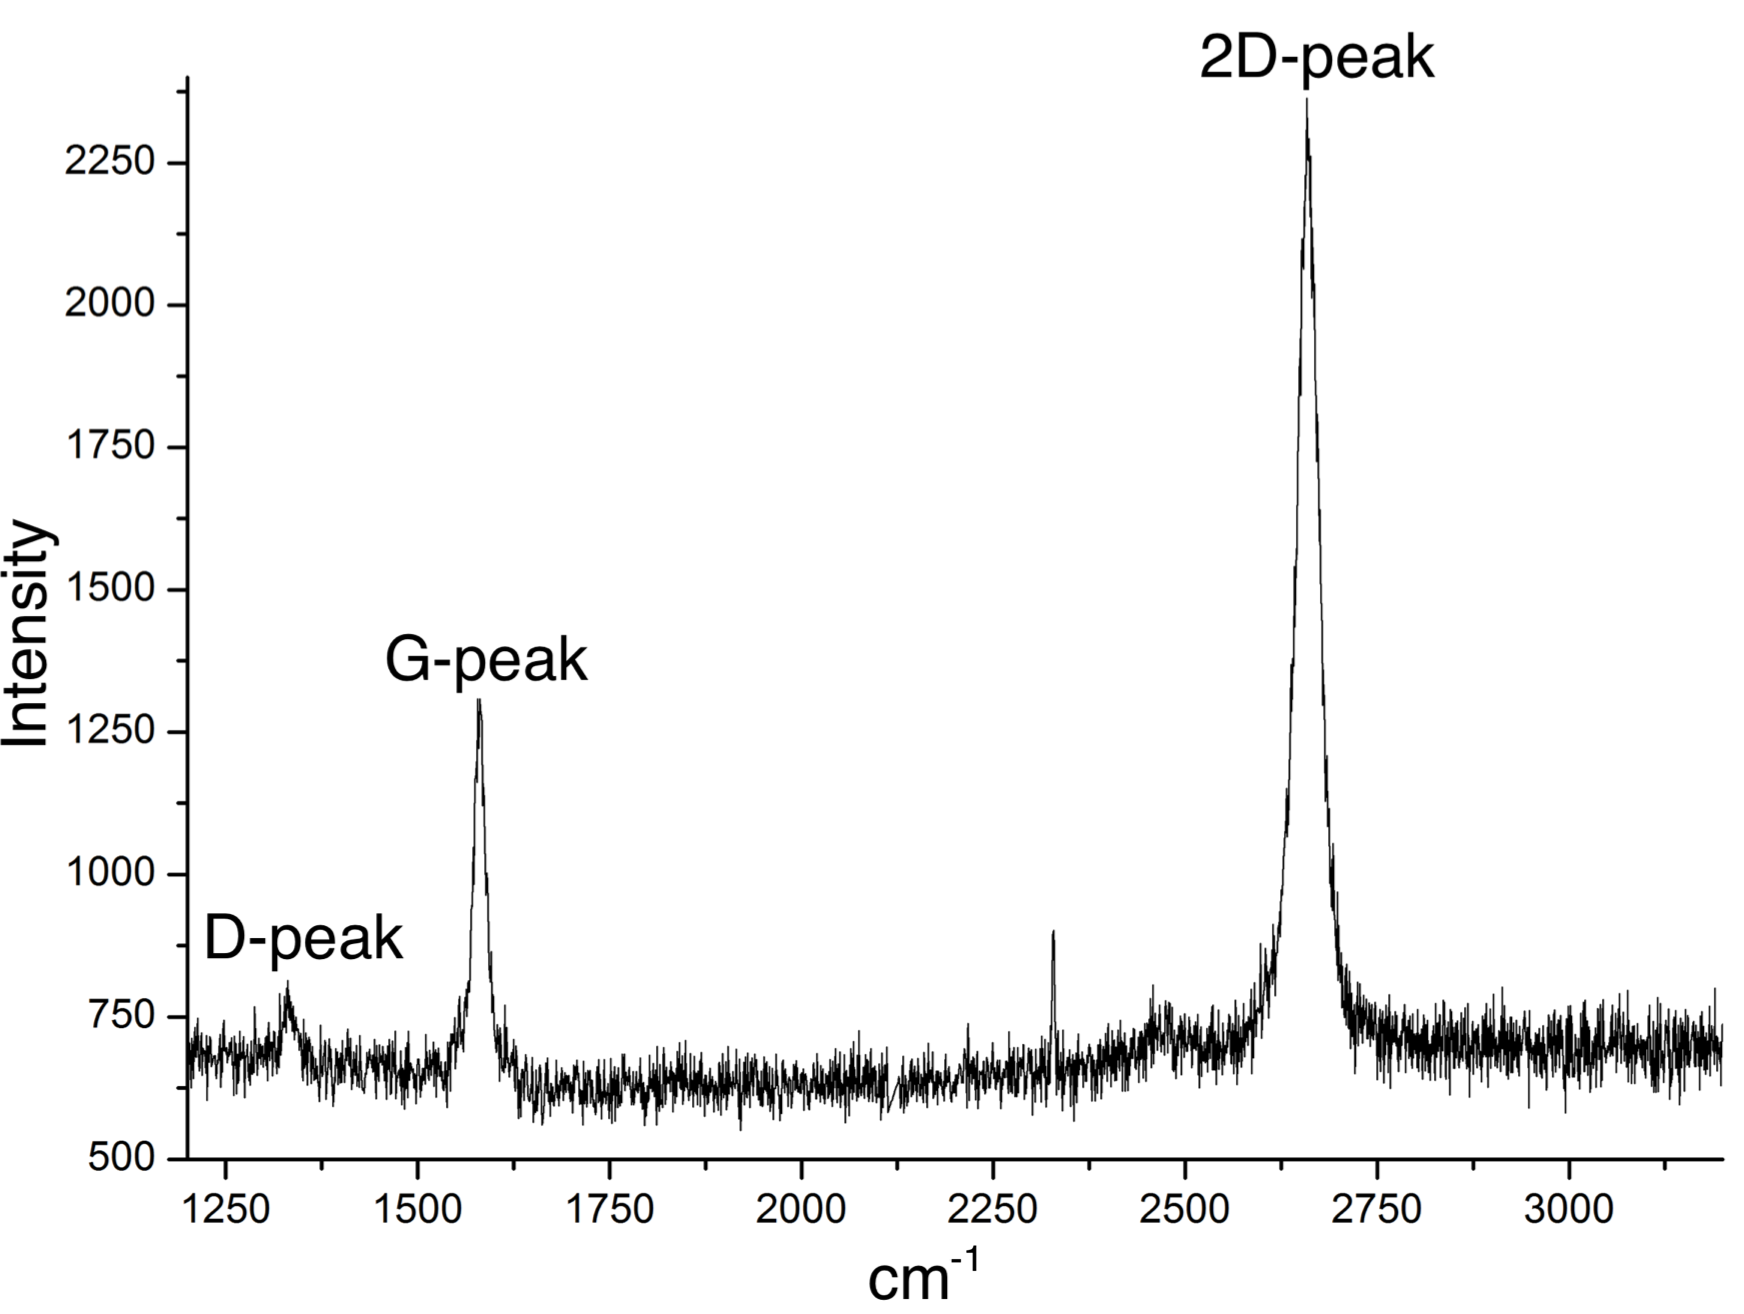
\includegraphics[width=\textwidth]{./images/graphene-raman.png}
  \end{subfigure}
  \caption{\textbf{(a)} Calculated phonon dispersion relation of graphene along the $\Gamma$-$K$-$M$-$\Gamma$-direction with six phonon branches (Figure adapted from Malard et al. 2009\mcite). \textbf{(b)} (adapted from \mcite).}
\end{figure}

\begin{figure}[!h]
  \centering
  \begin{subfigure}{0.3\textwidth}
    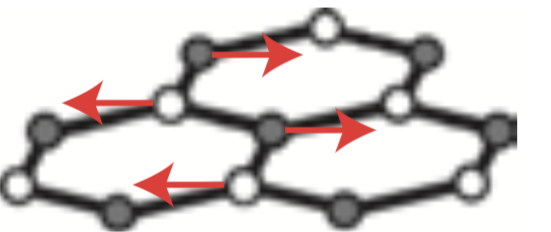
\includegraphics[width=\textwidth]{./images/g-mode-phonon.png}
  \end{subfigure}
  ~
  \begin{subfigure}{0.3\textwidth}
    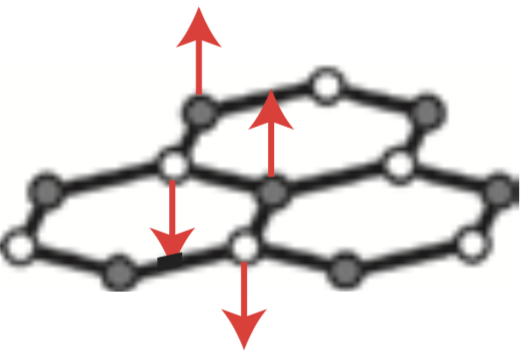
\includegraphics[width=\textwidth]{./images/g-mode-phonon-2.png}
  \end{subfigure}
  \begin{subfigure}{0.3\textwidth}
    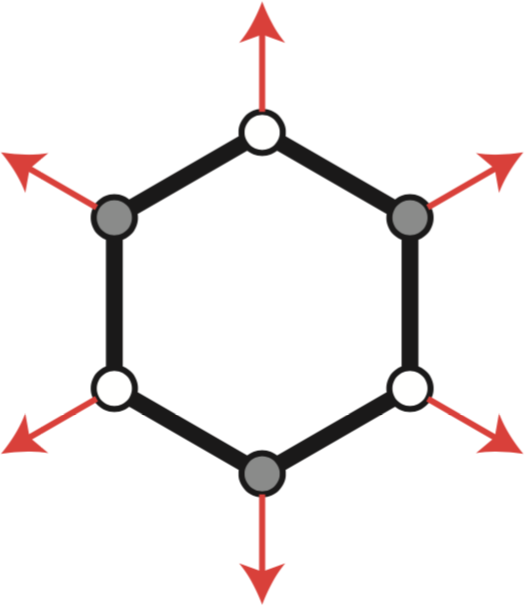
\includegraphics[width=\textwidth]{./images/2d-mode-phonon.png}
  \end{subfigure}
  \caption{\textbf{(a)} $\Gamma$ point displacement pattern for graphene, causing the $G$-peak in graphene's Raman spectrum. \textbf{(c)} Displacement at $K$ causing the $2D$-peak in graphene's Raman spectrum.}
\end{figure}

\begin{figure}[!h]
  \centering
  \begin{subfigure}{0.2\textwidth}
    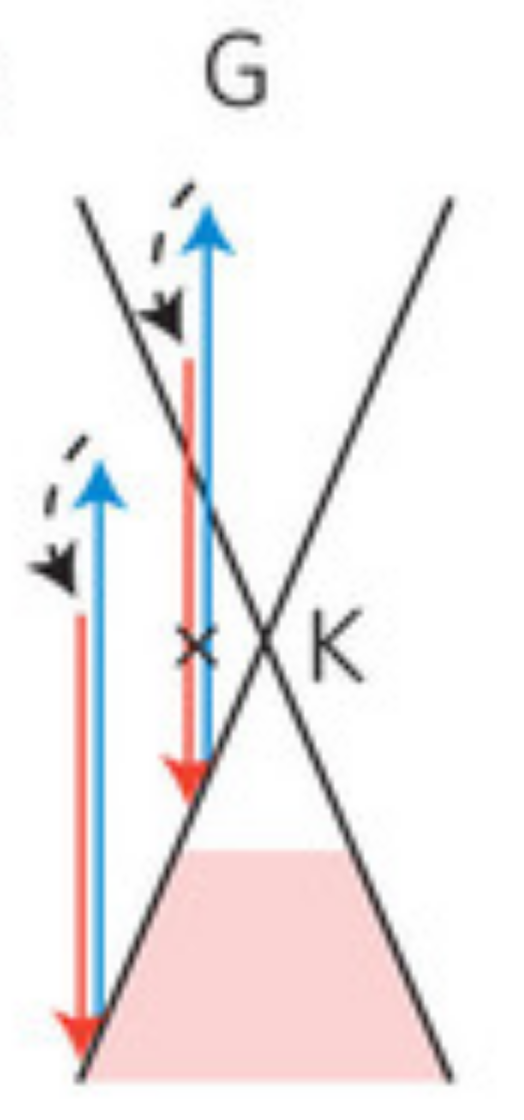
\includegraphics[width=\textwidth]{./images/g-mode.png}
  \end{subfigure}
  ~
  \begin{subfigure}{0.45\textwidth}
    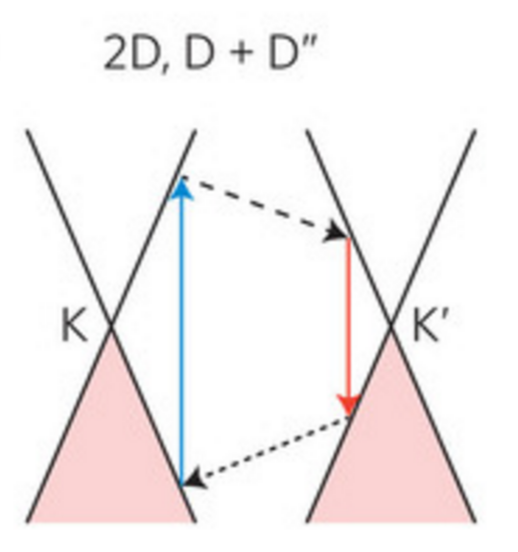
\includegraphics[width=\textwidth]{./images/2d-mode.png}
  \end{subfigure}
  \caption{\textbf{(a)} \textbf{(b)} }
\end{figure}

\subsubsection{Electromagnetic Enhancement Theory}

$$Enh_{local}(\mathbf{r},\omega_L)=\frac{\left|\mathbf{E}_{loc}(\mathbf{r}, \omega_L)\right|^2}{\left|\mathbf{E}_0\right|^2}\frac{\left|\mathbf{E}_{loc}(\mathbf{r}, \omega_L-\omega_{ph})\right|^2}{\left|\mathbf{E}_0\right|^2}\approx\frac{\left|\mathbf{E}_{loc}(\mathbf{r})\right|^4}{\left|\mathbf{E}_0\right|^4}$$

\note{see plasmonics book, 159}
